\documentclass[pi.tex]{subfile}
\begin{document}
\tikzstyle{menu}=[rectangle, draw=black, rounded corners, fill=blue!40,
        text centered, anchor=north, text=white, text width=4cm]
\tikzstyle{arrow}=[->, >=open triangle 90, thick]
\tikzstyle{line} = [draw, -latex']

\chapter{PERANCANGAN DAN IMPLEMENTASI}
Dalam bab ini akan dijelaskan lebih lanjut mengenai bagaimana perancangan dan implementasi bahasa pemrograman Haskell dalam pembuatan aplikasi desktop GUI menggunakan metode pemrograman FRP dan teknologi website.

\section{Gambaran Umum Aplikasi}
Seperti yang telah dijelaskan pada bab terdahulu, komputasi awan (\emph{cloud computing} atau biasa kita sebut \emph{cloud}  merupakan sebuah teknologi baru dalam dunia komputer khususnya dalam bidang sumber daya IT yaitu server. Hampir seluruh server yang digunakan oleh penyedia layanan teknologi informasi mulai memanfaatkan teknologi awan ini untuk mereduksi besaran biaya yang umumnya dikeluarkan apabila menggunakan arsitektur komputer tanpa awan. Di Indonesia, beberapa penyedia layanan IT baik berupa layanan ke konsumen maupun sesama penyedia jasa IT juga mulai melirik menggunakan teknologi awan ini. Sebagai contoh antara lain tokopedia.com, Go-Jek, bukalapak.com dan penyedia jasa IT lainnya berlomba-lomba untuk melakukan reduksi biaya yang timbul agar mendapat keuntungan maksimal dengan memindahkan sebagian infrastruktur IT nya ke layanan awan.

Selain dari sisi pengguna layanan komputasi awan, penyedia jasa komputasi awan publik sampai saat ini mulai tumbuh dan bersaing satu dengan lainnya untuk menarik perhatian konsumennya. Penyedia jasa komputasi awan publik antara lain, Amazon AWS, Google Cloud, Alibaba Cloud, yang berbasis penggunaan perjam, maupun DigitalOcean, Vultr, CloudKilat, yang berbasis penggunaan perbulan. Dalam penulisan kali ini yang jadi pembahasan adalah mengenai Amazon AWS atau dapat dikenal juga dengan nama \emph{Amazon Web Service}.

Jasa yang dihitung pada Aplikasi adalah jasa yang masuk ke dalam jenis \emph{On-Demand} yaitu jasa yang pembayarannya dibebankan kepada pengguna sesuai dengan jumlah lama penggunaan atas jasa tersebut. Dengan Aplikasi ini, pengguna pemula diharapkan tidak memerlukan koneksi internet maupun mendaftar sebagai member AWS untuk mengetahui estimasi biaya jasa AWS yang ingin digunakan.

Aplikasi bersifat dinamis, yaitu kalkulasi dilakukan secara \emph{real-time} pada saat pengguna menginput parameter-parameter terhadap atribut jasa AWS yang digunakan. Perhitungan secara \emph{real-time} ini menggunakan konsep FRP yang ada pada pustaka Reflex dan Reflex-Dom, sehingga pembaharuan terhadap DOM berupa hasil kalkulasi terlihat terjadi seketika.

\section{Kebutuhan Perangkat dan Instalasi Aplikasi}
Dalam Penulisan Ilmiah ini, tidak semua perangkat komputer dapat menjalankannya. Hal ini dipengaruhi oleh spesifikasi perangkat keras \emph{hardware} dan spesifikasi perangkat lunak \emph{software} mesin tempat dimana Aplikasi akan dijalankan.

Selain dar kebutuhan perangkat, Aplikasi tidak dapat langsung digunakan, melainkan harus melalui tahapan instalasi terlebih dahulu. Kebutuhan akan penjelasan bagaimana cara melakukan instalasi Aplikasi di sebuah mesin yang sudah dianggap sesuai dengan spesifikasi minimal sangat diperlukan untuk meminimalisir kesalahan pada saat aplikasi dijalankan.

Oleh karena itu, berikut ini akan dijelaskan apa saja kebutuhan perangkat dan bagaimana cara melakukan instalasi Aplikasi di sebuah sistem operasi.
\subsection{Kebutuhan Minimal dan Maksimal Perangkat}
Kebutuhan minamal perangkat keras dan lunak untuk menjalankan Aplikasi adalah sebagai berikut:

\begin{table}[h]
  \centering
\begin{tabular}{ |p{3cm}||p{6cm}|}
  
  \hline
  \multicolumn{2}{|c|}{Minimum Requirement} 
  \\ \hline
  Name & Specification \\
  \hline
  Sistem Operasi : & macOS Sierra \\
  Processor : & 2.4 GHz Intel Core 2 Duo \\
  Memory : & 4GB \\
  Graphics : & NVIDIA GeForce 320M 256MB \\
  \hline
  
\end{tabular}
\caption{Kebutuhan Minimal}
\end{table}

Kebutuhan minimal diperlukan agar pengguna mengetahui apakah perangkat yang dimilikinya mampu untuk menjalankan Aplikasi. Kemampuan Aplikasi berjalan pada spesifikasi perangkat pada tingkat minimal menunjukkan bahwa jalannya Aplikasi tidak akan mengganggu atau membuat aktivitas perangkat menjadi terganggu.

\begin{table}[h]
  \centering
\begin{tabular}{ |p{3cm}||p{6cm}|}
  \hline
  \multicolumn{2}{|c|}{Recommended Requirement} 
  \\ \hline
  Name & Specification \\
  \hline
  Sistem Operasi : & macOS Sierra \\
  Processor : & 2.8 GHz Intel Core i7 \\
  Memory : & 16GB \\
  Graphics : & NVIDIA GeForce GT 750M 2048MB \\
  \hline
  
\end{tabular}

\caption{Kebutuhan Yang Direkomendasikan}
\end{table}

Kebutuhan yang direkomendasikan diperlukan agar baik pengguna maupun pengembang mengetahui perangkat mana yang dapat menghasilkan performa yang optimal ketika Aplikasi sedang dijalankan.

Dari kedua tabel diatas, sistem operasi berperan penting dalam penentuan spesifikasi sebuah Aplikasi. Hal ini dikarenakan apabila jenis perangkat keras telah terpenuhi namun sistem operasi tidak terpenuhi, Aplikasi tidak dapat dijalankan.


\subsection{Instalasi Aplikasi}
Instalasi Aplikasi dilakukan melalui beberapa tahapan, yaitu:
\subsubsection{Instalasi XCode dan XCode Command Line Tools}
  Instalasi XCode dapat dilakukan dengan membuka App Store pada menu dock MacOS (Letak dock ada dibagian bawah Desktop) kemudian cari aplikasi XCode pada menu pencarian dan pasang XCode pada MacOS dengan menekan tombol GET. Berikut adalah tampilan langkah pada gambar:
  
  \begin{figure}[H]
      \centering
  
\includegraphics{appStore}
  \caption[Ikon AppStore]{Ikon AppStore}

  \end{figure}

  \begin{figure}[H]
      \centering
  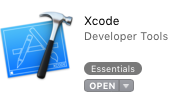
\includegraphics{xcode.png}
  \caption[Ikon XCode]{Ikon XCode}
  \end{figure}

  Setelah selesai melakukan instalasi, buka terminal MacOS dan ketikkan perintah 'xcode-select --install' pada terminal. Klik pada tombol install untuk melakukan instalasi xcode command line tools. Apabila telah berhasil terpasang, ketik perintah 'xcode-select -p' untuk memeriksa apakah xcode command line tools tersebut sudah terpasang atau belum.
  
\subsubsection{Instalasi GHC sebagai alat kompilasi dan Cabal sebagai manajemen paket}
  Untuk mamasang GHC pada MacOS, dapat dilakukan dengan cara mengunduh GHC melalui situs resminya yaitu \url{https://www.haskell.org/ghc/download_ghc_8_0_2.html} pada bagian \emph{Binary Package}. Downlod file binary untuk Mac OS X, dan jalankan installer dengan cara menekan mouse kiri pada binary sebanyak 2 (dua) kali. Ikuti langkah-langkah yang ditampilkan sampai dengan GHC berhasil terpasang.

  Untuk Cabal, pemasangan dapat dilakukan dengan mengunduh \url{https://www.haskell.org/cabal/download.html} dan pilih Cabal library serta cabal-install tools. Extract cabal-install dan jalankan shell script bernama \emph{bootstrap.sh} dimana skrip ini mengunduh dan memasang semua kebutuhan paket yang akan digunakan oleh program cabal-install
  
\subsubsection{Instalasi Aplikasi dari kode sumber}
  Unduh kode sumber dari Aplikasi di \url{https://github.com/Rizary/awspi} kemudian pindah kedalam direktori kode dengan mengetik 'cd awspi'. Setelah berhasil masuk kedalam folder kode sumber, jalankan perintah 'cabal new-build' untuk melakukan kompilasi terhadap kode sumber Aplikasi tersebut.

  Setelah proses kompilasi berhasil, file binary dari aplikasi akan terletak pada folder \url{./dist-newstyle/build/x86_64-osx/ghc-8.0.2/awspi-0.0.0.1/build/} dalam bentuk ekstensi '.app'. Klik 2 kali pada file tersebut untuk menjalankan Aplikasi. Aplikasi yang berhasil dijalankan akan tampak seperti gambar dibawah ini:
  
  \begin{figure}[H]
    \centering
  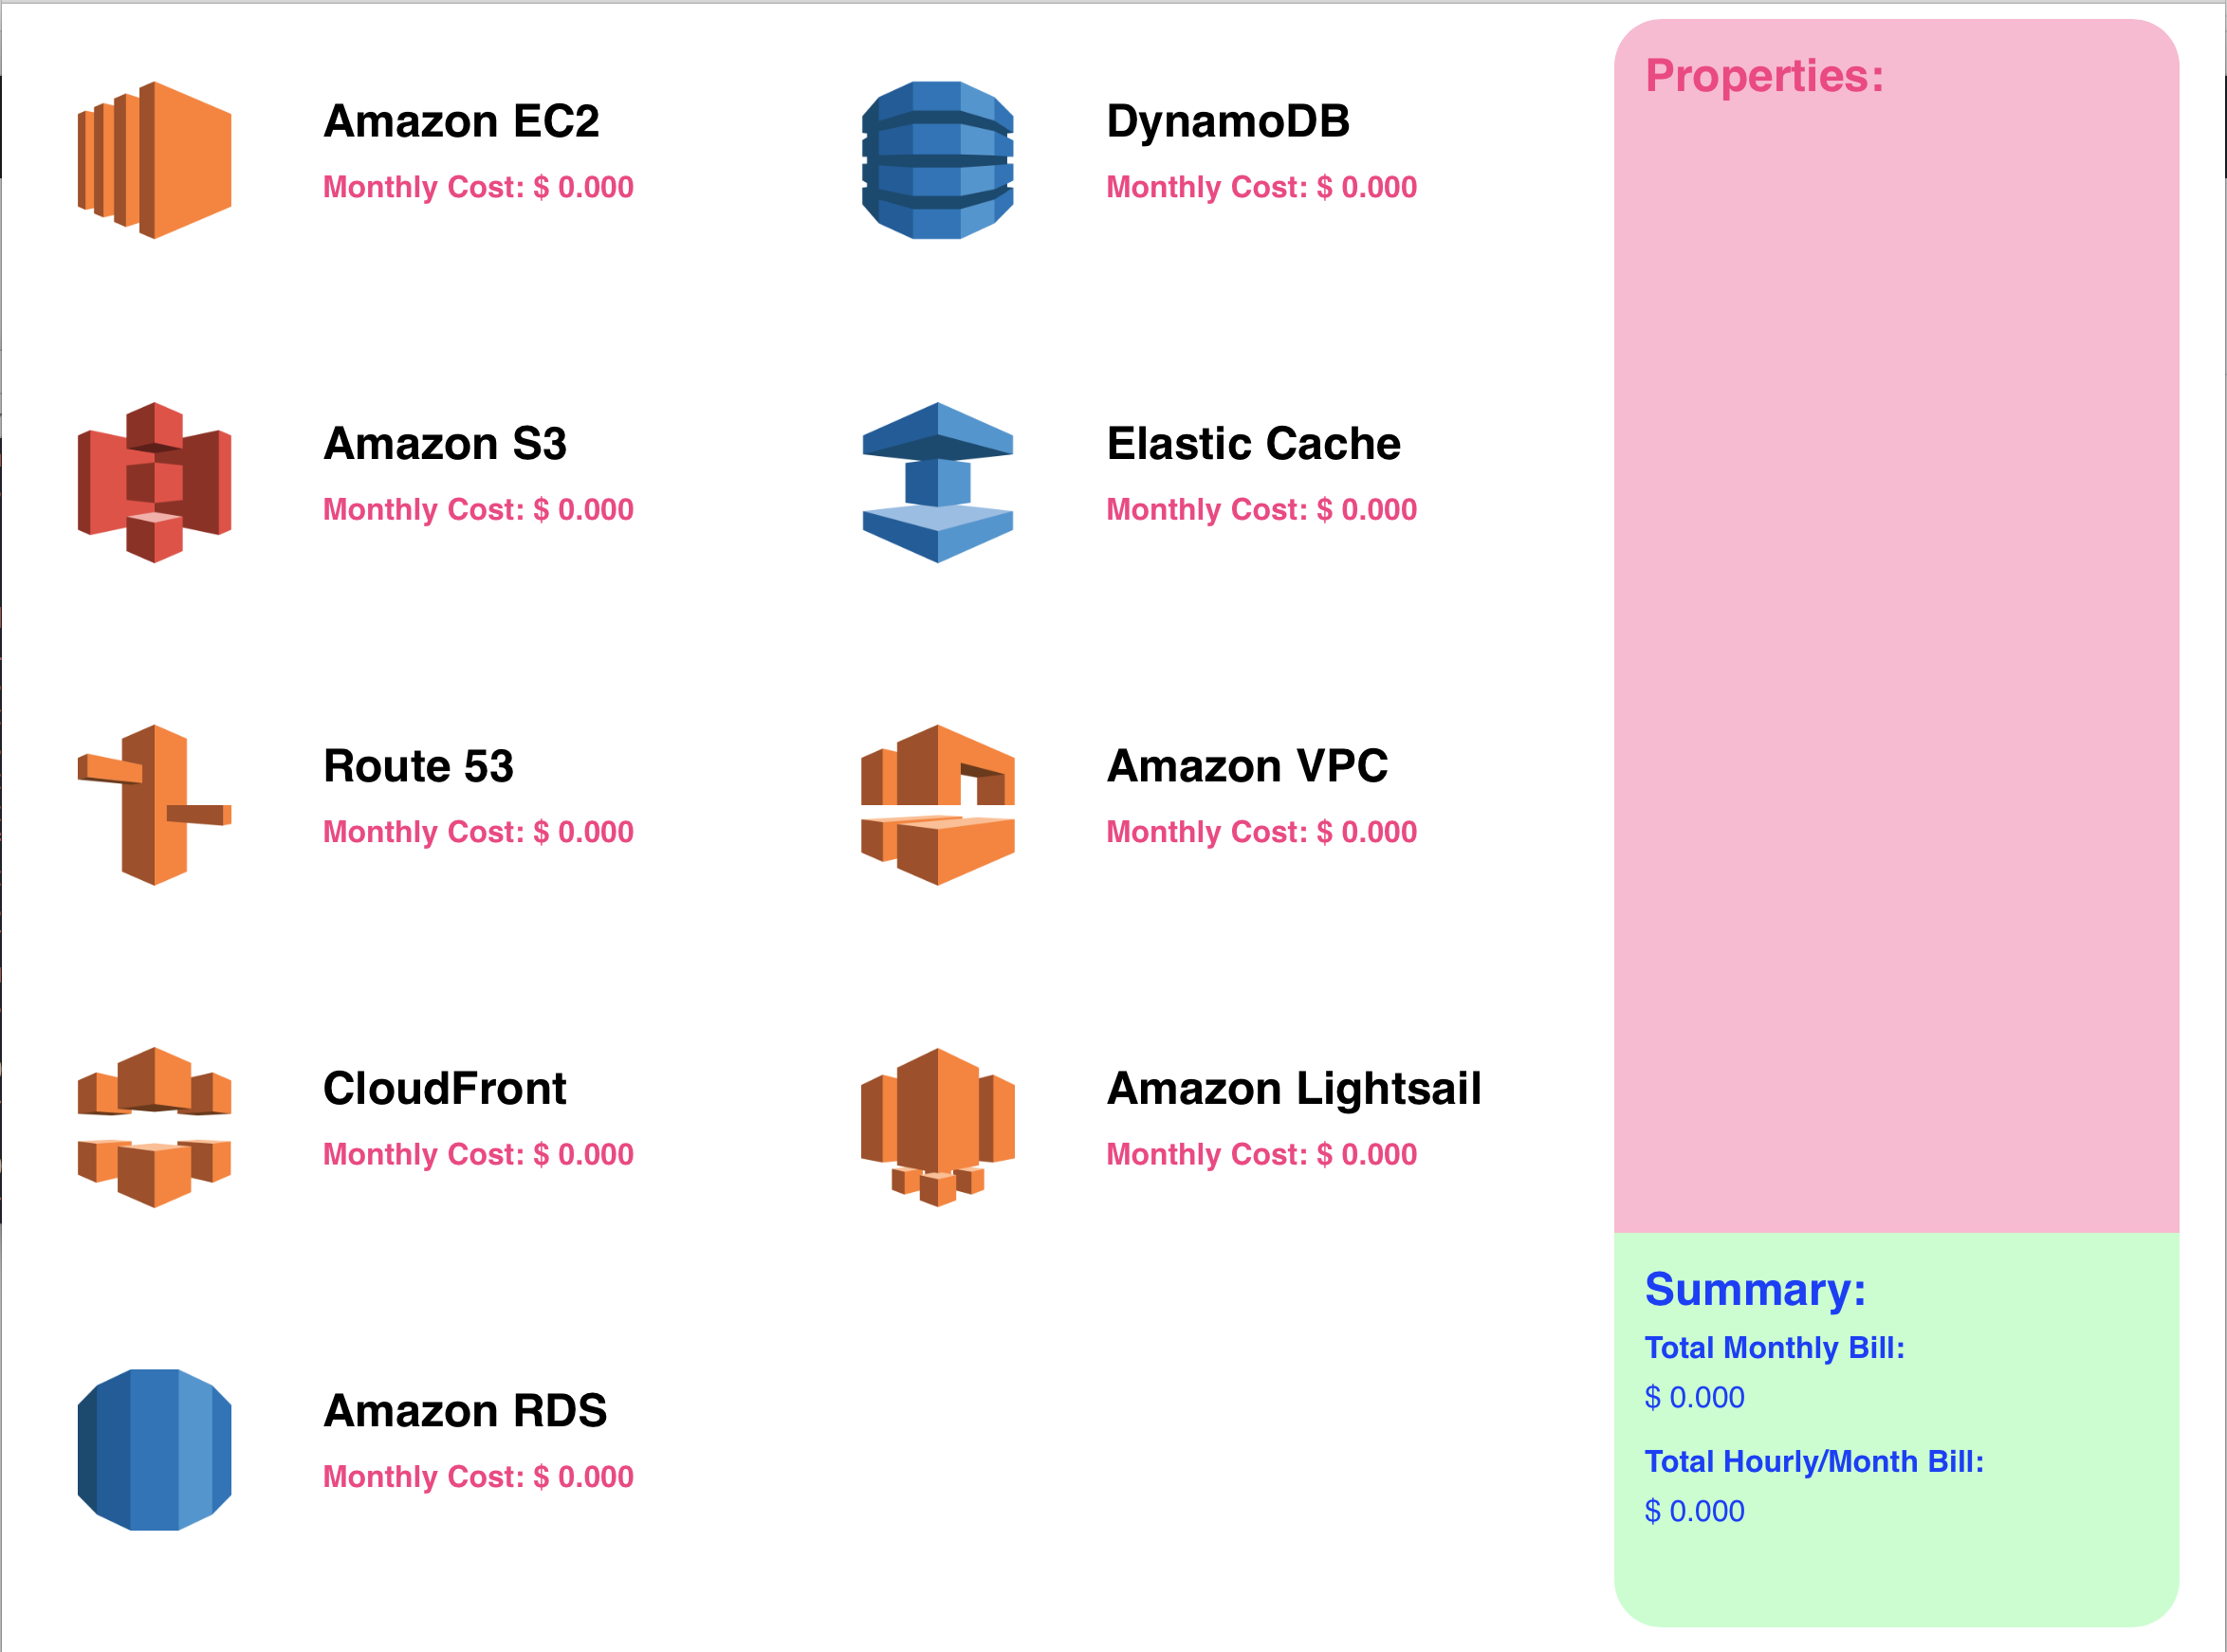
\includegraphics[width=15cm, height=10cm]{awspi.png}
  \caption[Tampilan Awal Aplikasi]{Tampilan Awal Aplikasi}
  \end{figure}

  Apabila sudah sesuai dengan gambar diatas, maka Aplikasi sudah dapat digunakan.

\section{Tahapan Pembuatan Dan Algoritma Aplikasi}
\subsection{Tahapan Pembuatan Aplikasi}
Dalam membuat Aplikasi, tahapan yang dilakukan adalah merancang dan membuat desain. Perancangan Aplikasi pada penulisan ilmiah ini adalah menggunakan struktur navigasi non-linier, sebagaimana digambarkan sebagai berikut:

\begin{figure}[H]
  \centering
  \begin{tikzpicture}[node distance=2cm]
    \node (main)[menu]
          {
            \textbf{Menu Utama}
          };
    \node (RDS)[menu,below of=main]
          {
            \textbf{Properti \\ Amazon RDS}
          };
    \node (CF)[menu,left of=RDS, xshift=-4cm]
          {
            \textbf{Properti CloudFront}
          };
    \node (R53)[menu,below of=CF]
          {
            \textbf{Properti Route53}
          };
    \node (S3)[menu,below of=R53]
          {
            \textbf{Properti Amazon S3}
          };
    \node (EC2)[menu,below of=S3]
          {
            \textbf{Properti \\ Amazon EC2}
          };          
    \node (DDB)[menu,right of=RDS, xshift=4cm]
          {
            \textbf{Properti \\ DynamoDB}
          };
    \node (EC)[menu,below of=DDB]
          {
            \textbf{Properti \\ ElasticCache}
          };
    \node (VPC)[menu,below of=EC]
          {
            \textbf{Properti \\ Amazon VPC}
          };
    \node (LS)[menu,below of=VPC]
          {
            \textbf{Properti \\ Amazon LightSail}
          };

          \path[line] (main.south) -- (RDS.north);
          \path[line] (main.west) -- ++(0,0) -| (CF.west);
          \path[line] (main.west) -- ++(0,0) -| (R53.west);
          \path[line] (main.west) -- ++(0,0) -| (S3.west);
          \path[line] (main.west) -- ++(0,0) -| (EC2.west);
          \path[line] (main.east) -- ++(0,0) -| (DDB.east);
          \path[line] (main.east) -- ++(0,0) -| (EC.east);
          \path[line] (main.east) -- ++(0,0) -| (VPC.east);
          \path[line] (main.east) -- ++(0,0) -| (LS.east);
          
  \end{tikzpicture}
  \caption[Struktur Navigasi Aplikasi]{Struktur Navigasi Aplikasi AWS}
\end{figure}

Dari struktur navigasi diatas, menu utama menggambarkan ikon-ikon jasa AWS yang dapat dipilih. Contoh menu utama dalam desain adalah sebagai berikut:

  \begin{figure}[H]
      \centering
  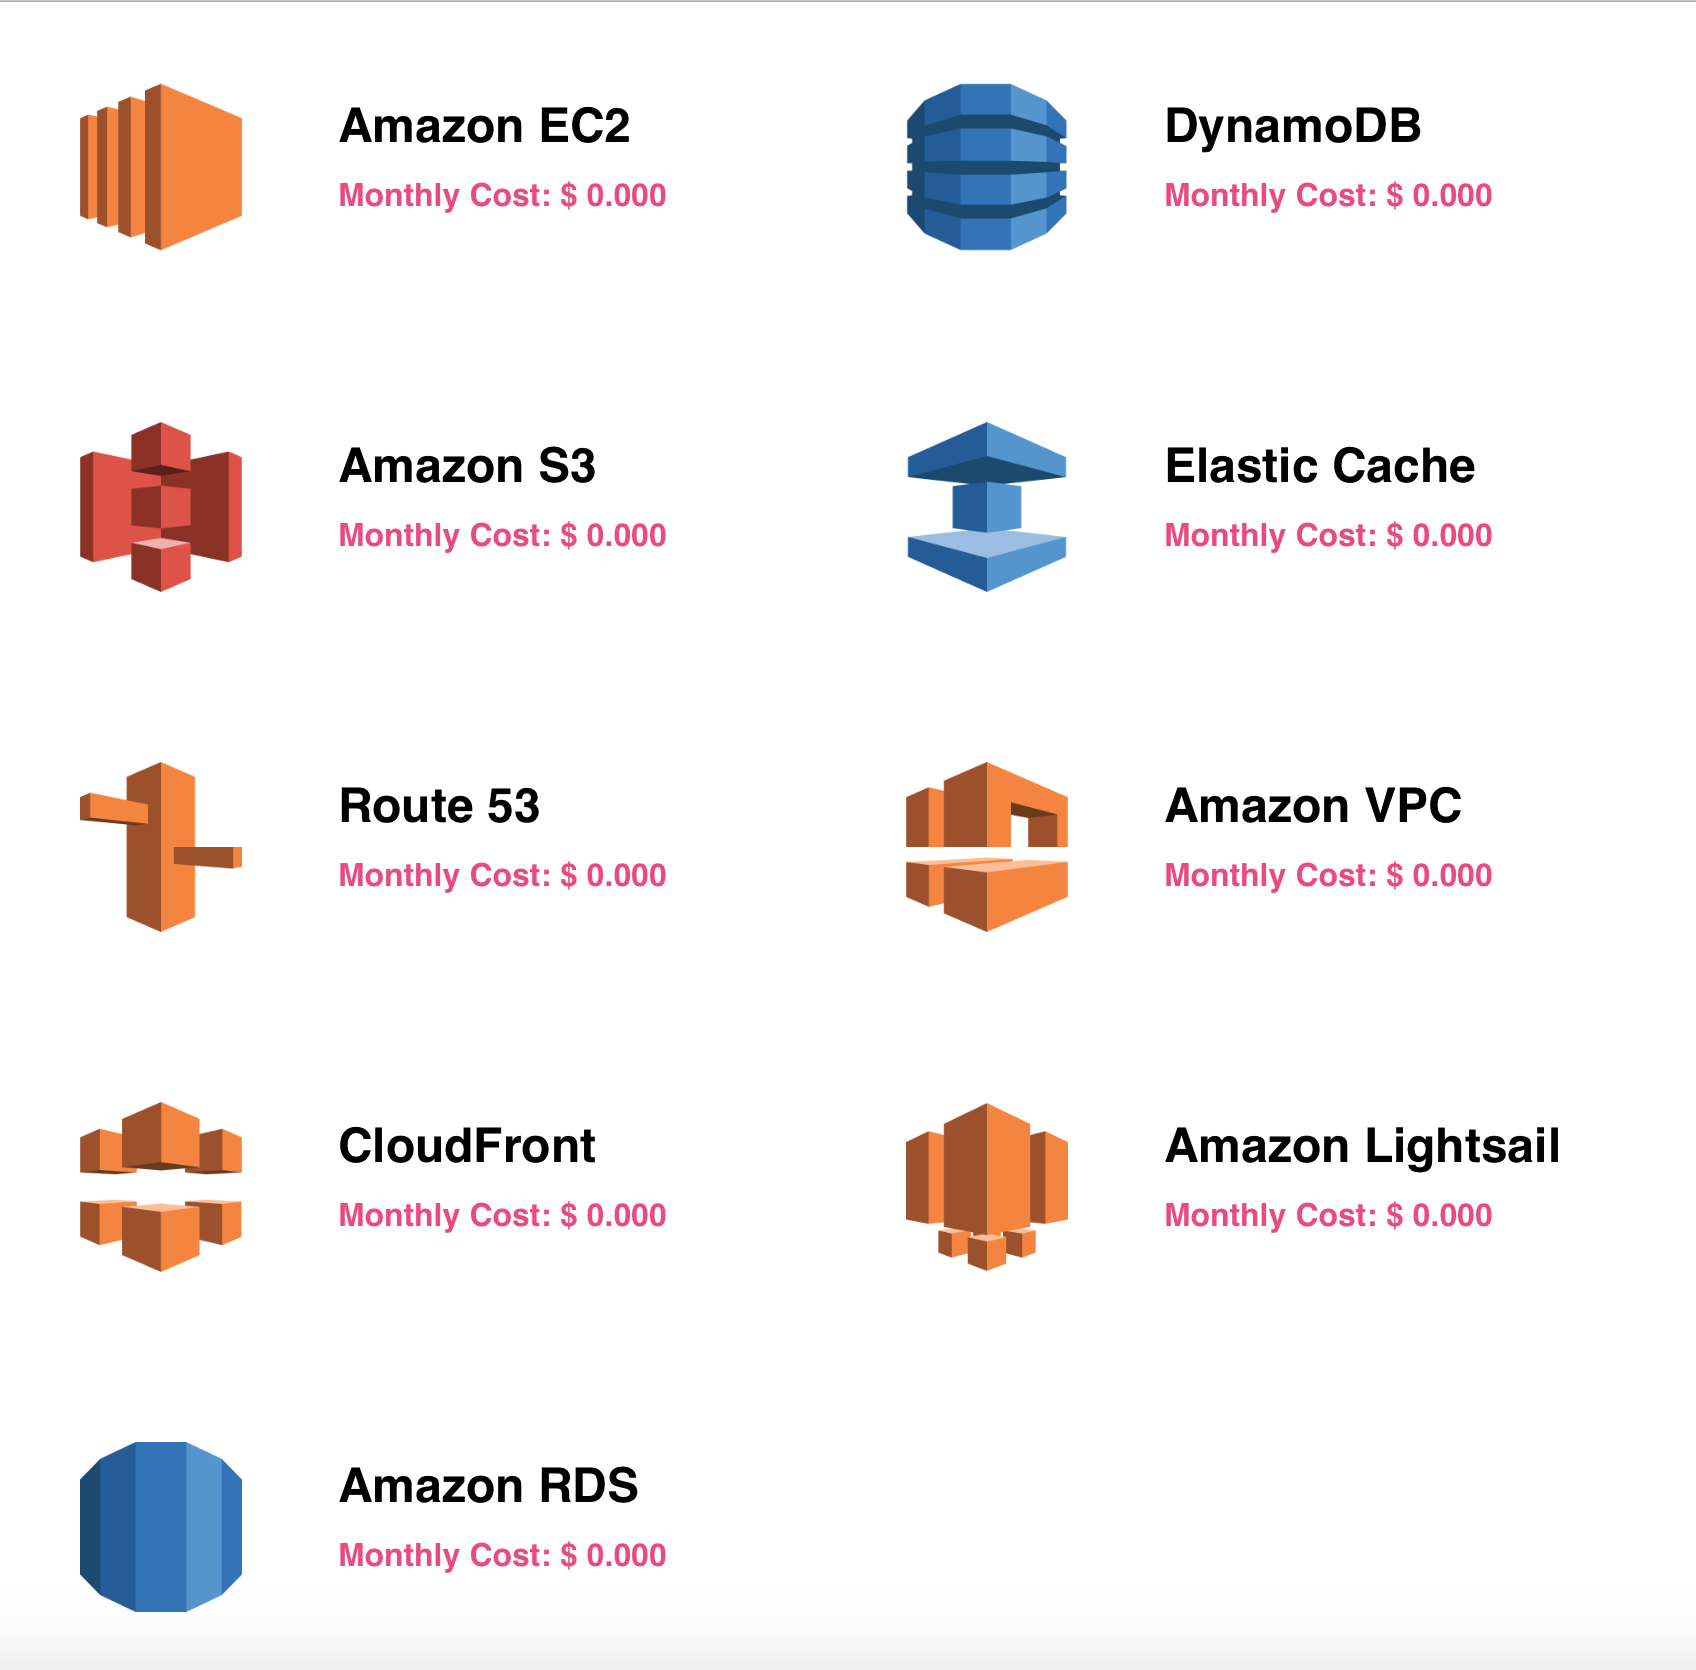
\includegraphics[width=10cm, height=10cm]{aws3.png}\\
  \caption[Menu Utama Aplikasi]{Menu Utama Aplikasi AWS}
  \end{figure}

  Menu utama merupakan acuan untuk menampilkan menu properties yang terletak di sebelah kanan Aplikasi, seperti pada gambar dibawah ini:
    \begin{figure}[H]
      \centering
  
\includegraphics[width=8cm, height=10cm]{aws4.png}\\
  \caption[Menu Properties Aplikasi]{Menu Properties Aplikasi AWS}
  \end{figure}

    Menu summary tidak dapat berubah, sehingga bersifat statis mengikuti menu utama. Dengan demikian, struktur navigasi yang sesuai untuk pembuatan aplikasi ini adalah non-linier karena dalam struktur ini terdapat percabangan, namun tidak adanya master maupun slave pada halaman tersebut.

    Untuk desain Aplikasi, penelitian ilmiah ini menggunakan aplikasi pendukung prototipe bernama Sketch pada MacOS dengan menggunakan metode desain 8pt (\emph{8pt Design}), yaitu jarak spasi antara satu ikon / gambar dengan yang lainnya berjarak 8 point atau kelipatan 8 (termasuk didalamnya kelipatan 2 dan 4). Hal ini akan memudahkan dalam penggunaan di dalam beberapa resolusi layar. Hasil final terhadap desain adalah sebagai berikut:
    \begin{figure}[H]
      \centering
  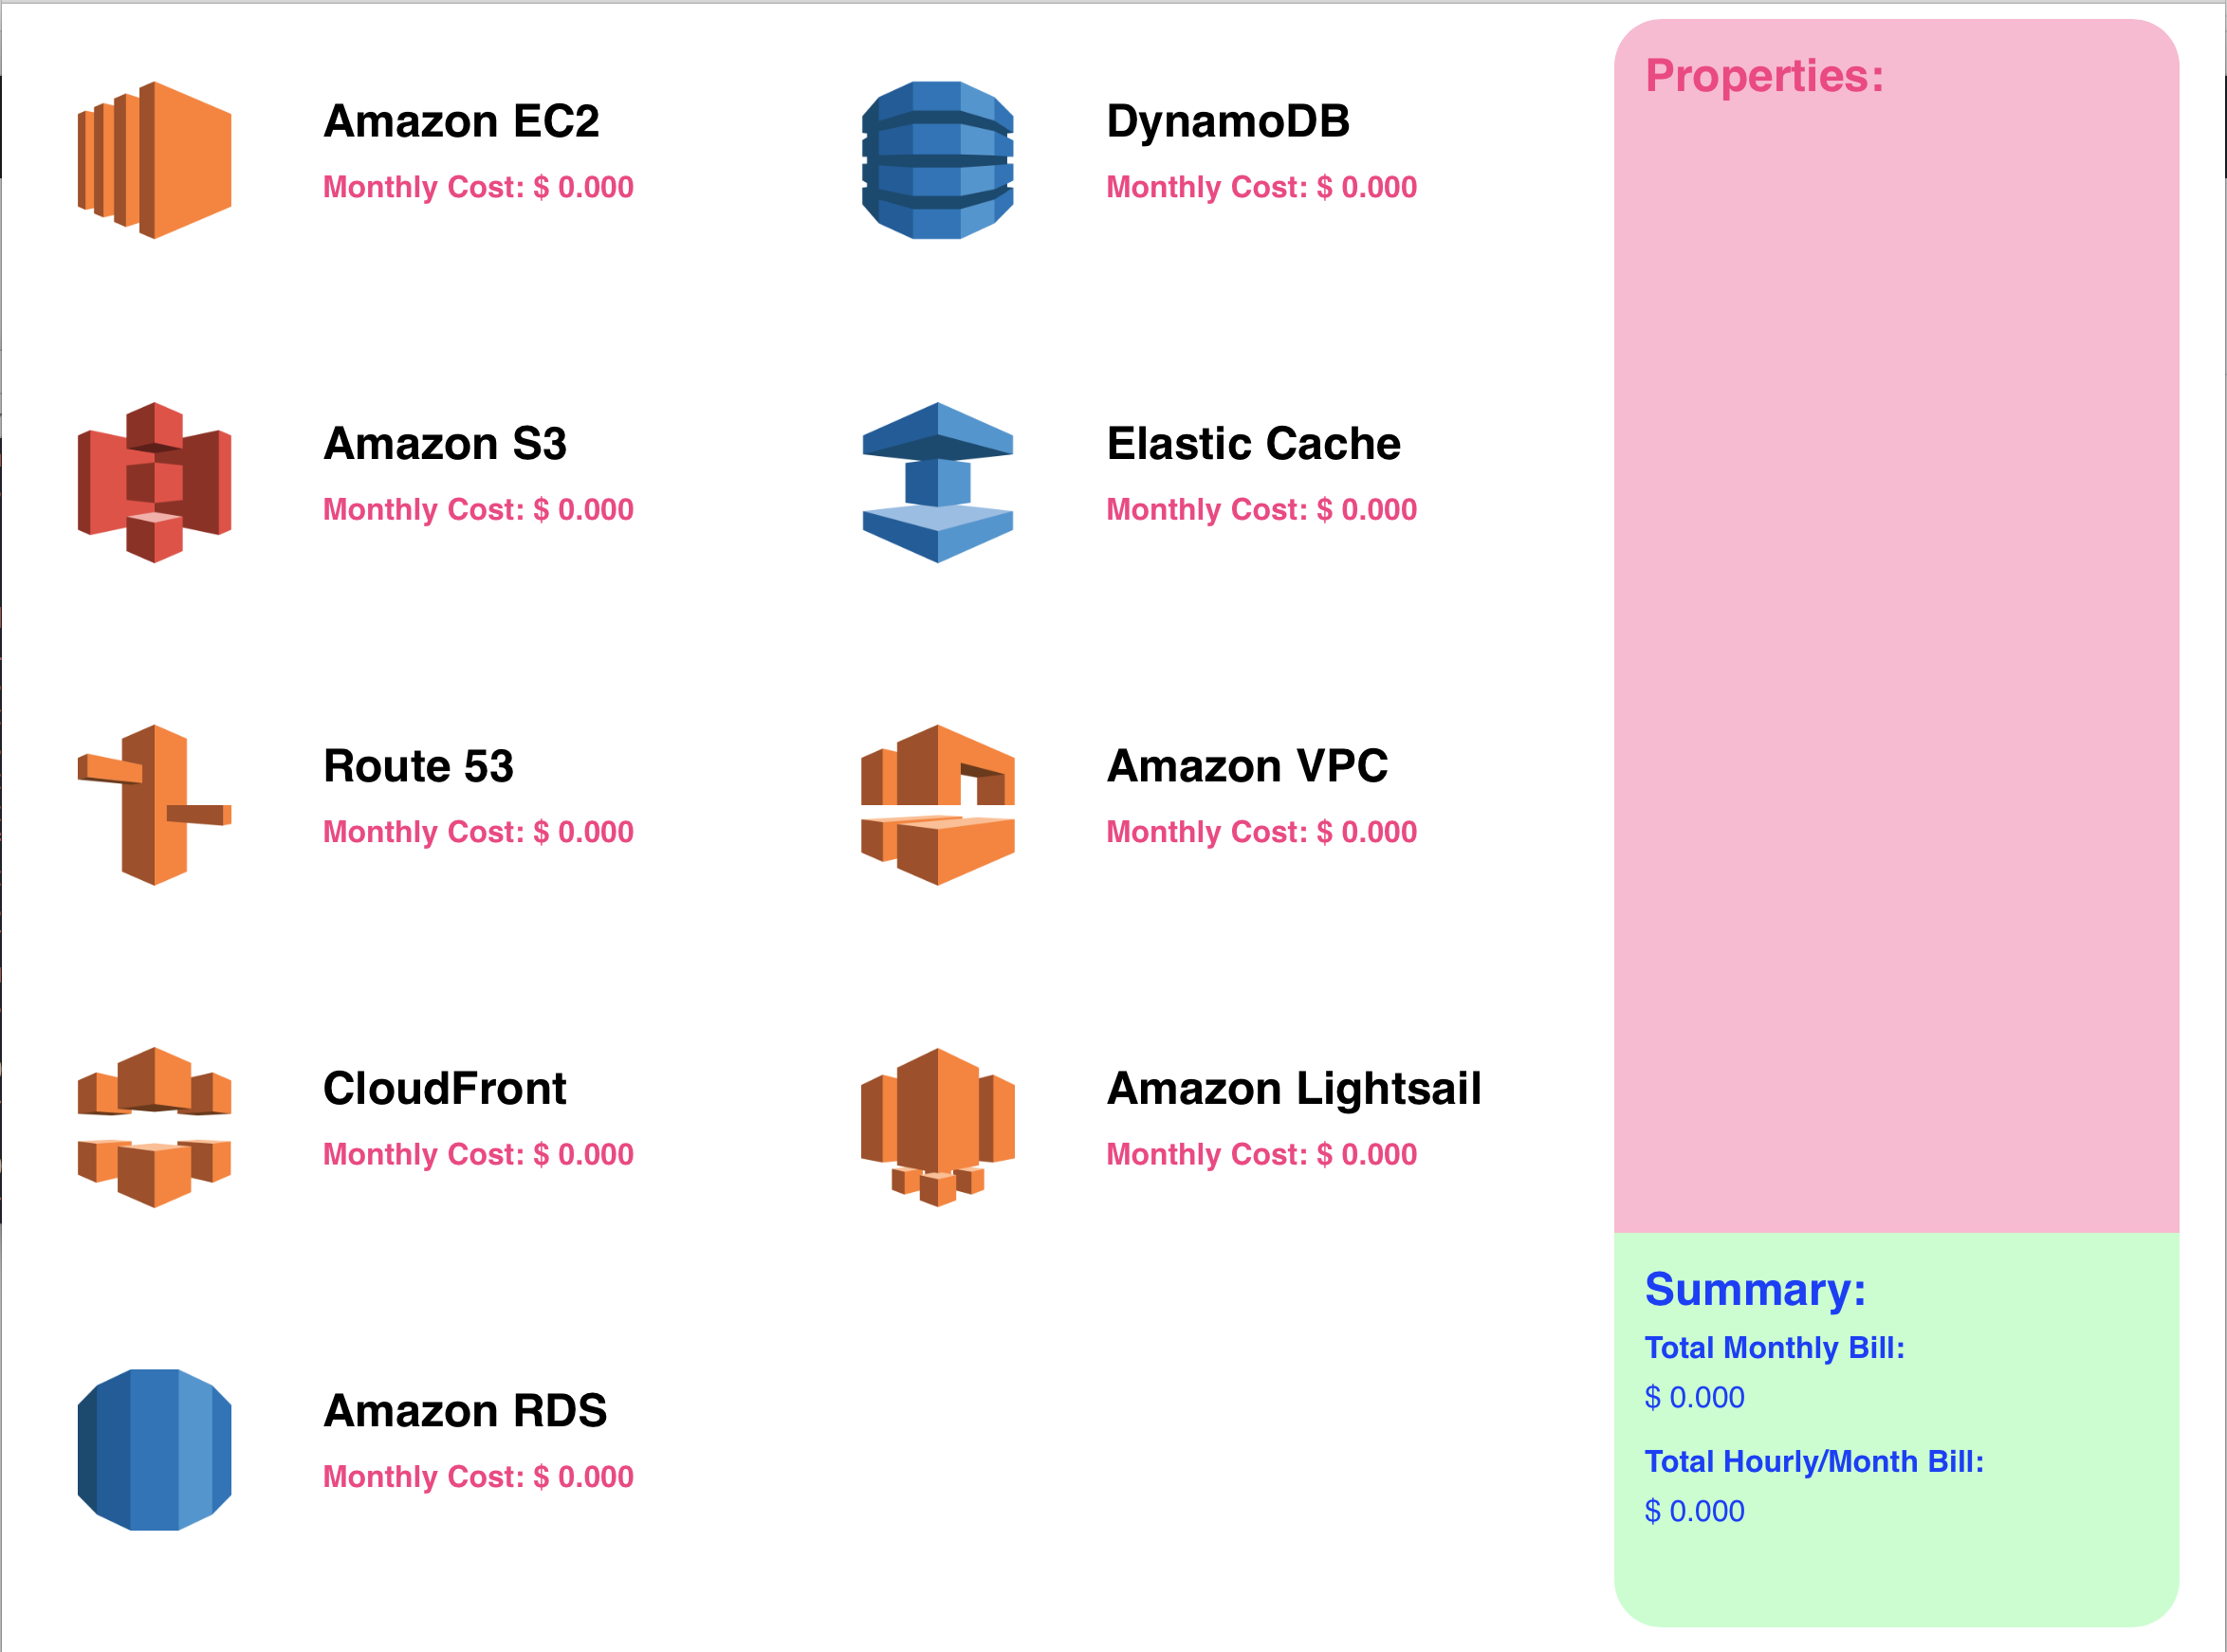
\includegraphics[width=15cm, height=10cm]{awspi.png}\\
  \caption[Tampilan Awal Aplikasi Berjalan]{Tampilan Awal Aplikasi Berjalan}
    \end{figure}

    \begin{figure}[H]
      \centering
  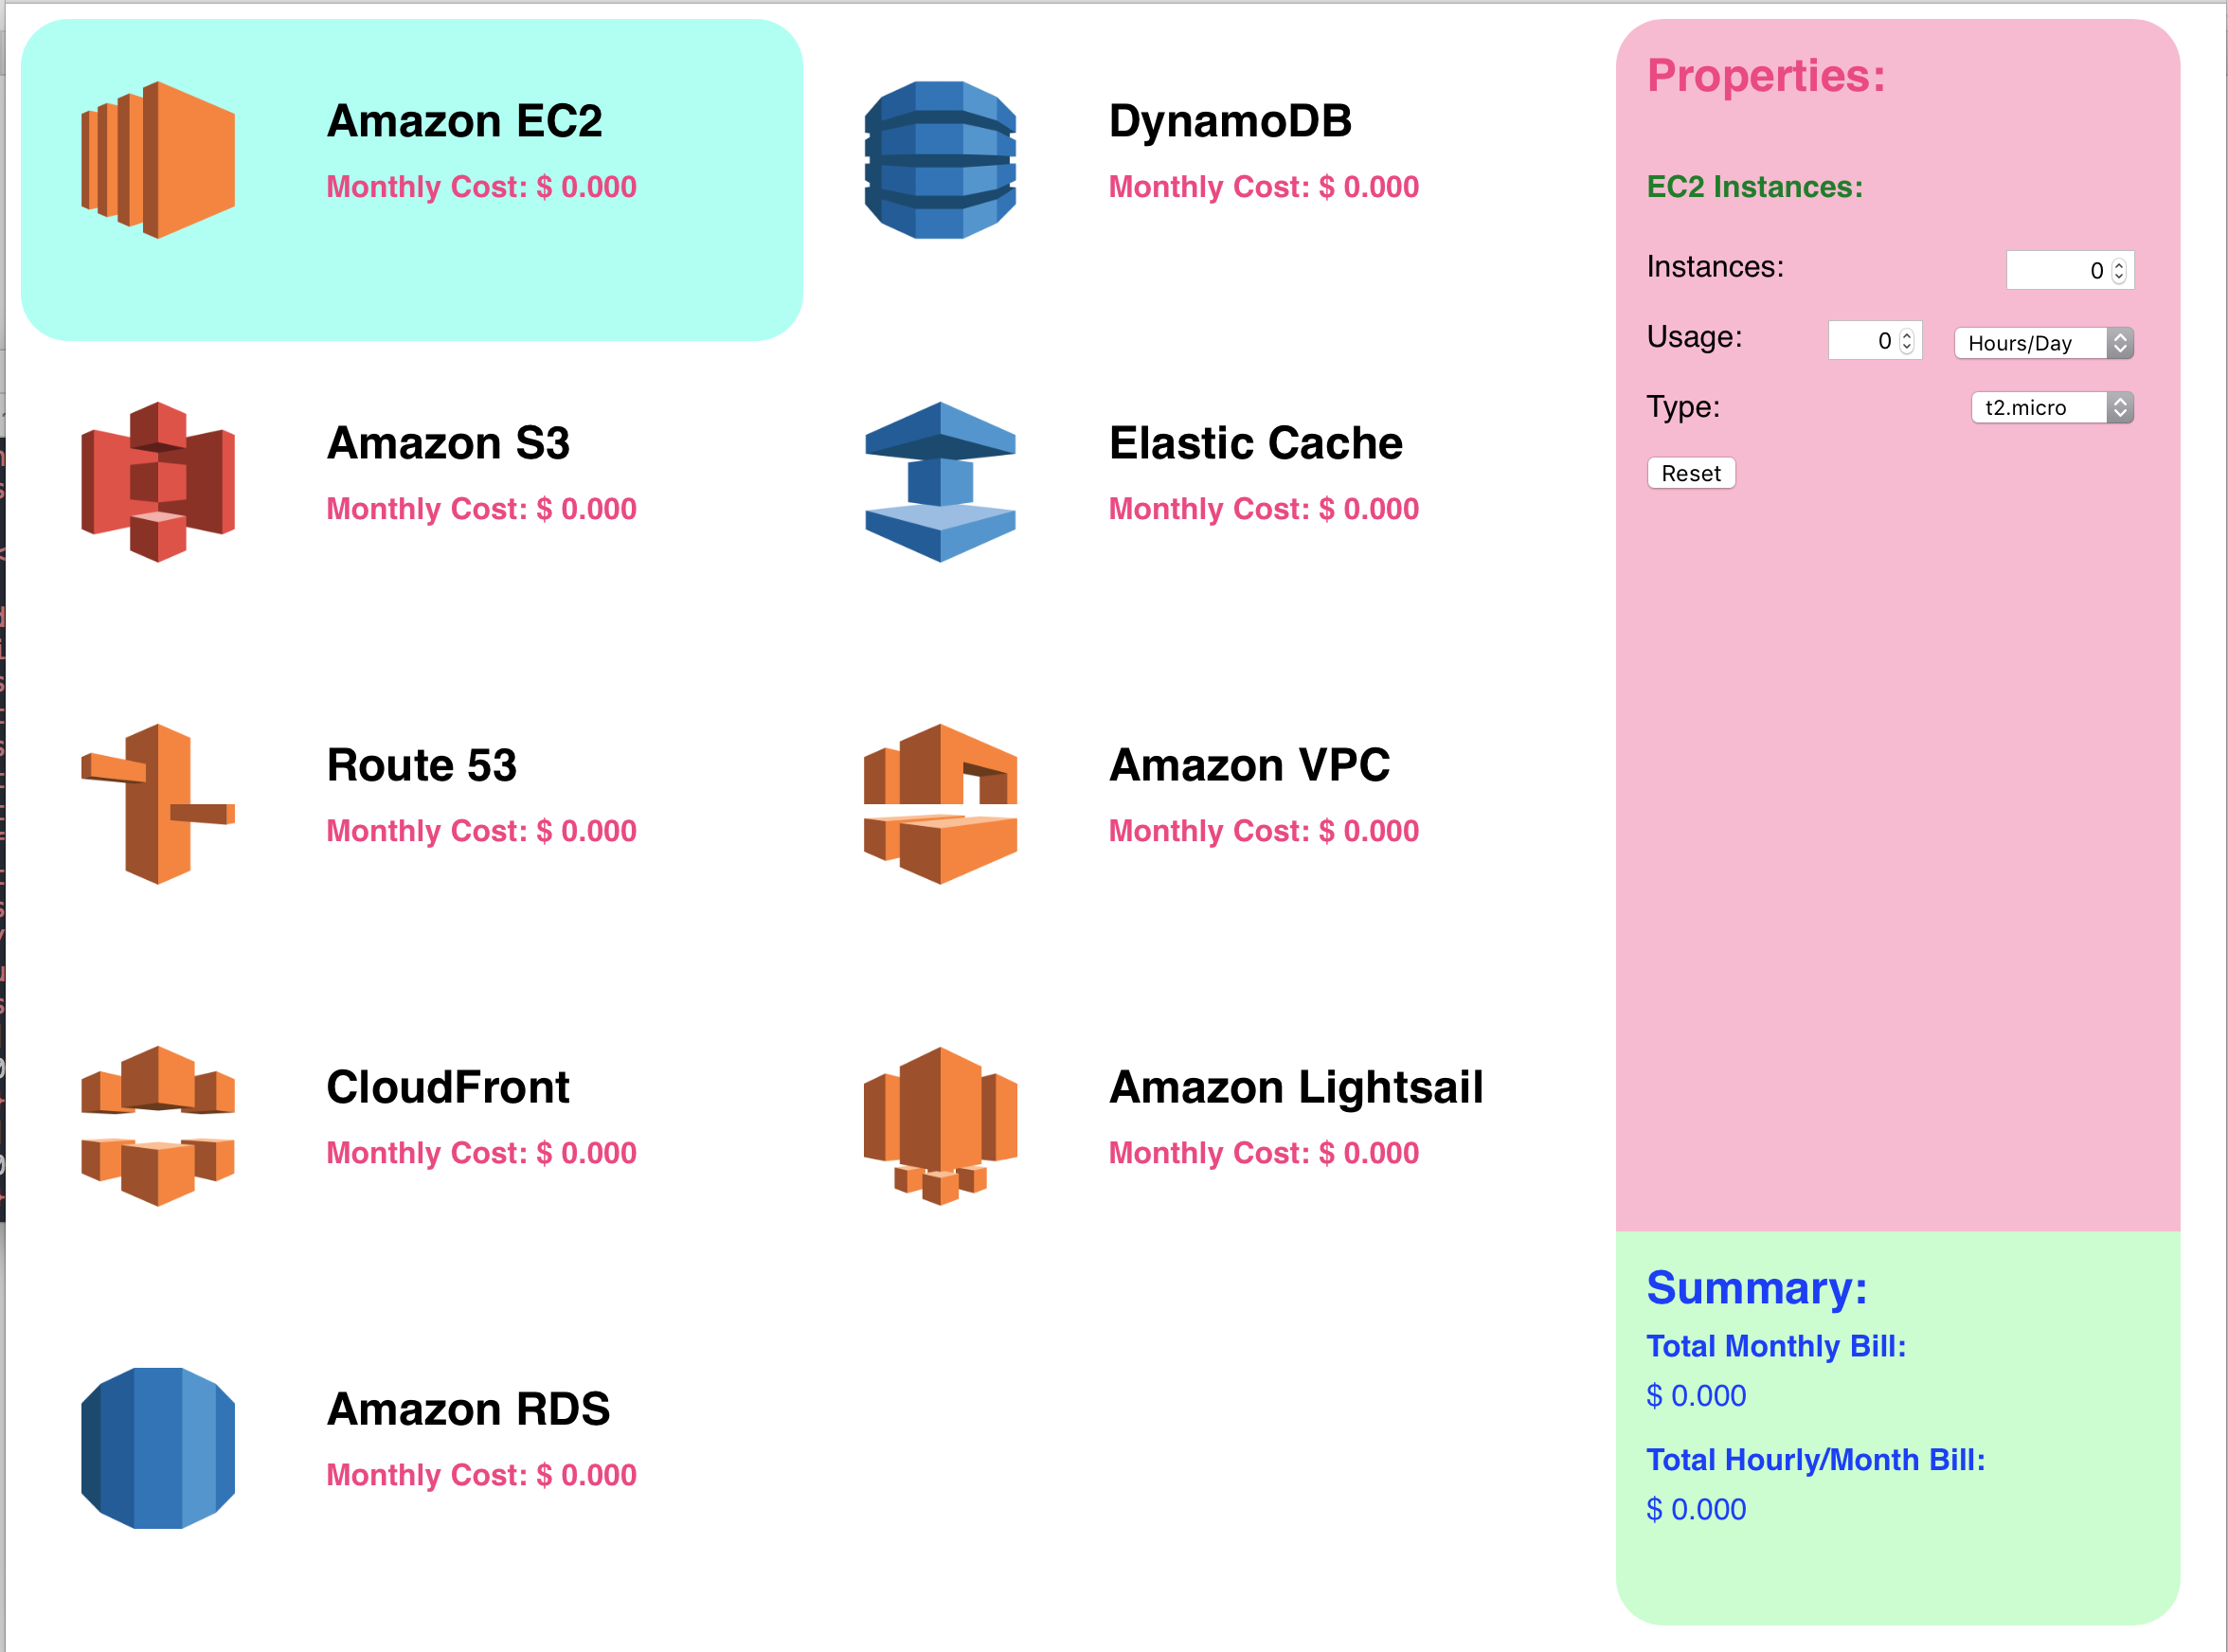
\includegraphics[width=15cm, height=10cm]{aws2.png}\\
  \caption[Tampilan Seleksi Menu]{Tampilan Ketika Salah Satu Menu Terseleksi}
    \end{figure}


\subsection{Algoritma Aplikasi}
Aplikasi pertama kali dijalankan melalui fungsi main yang ada pada file Main.hs. Main.hs terletak di folder \url{./frontend/Main.hs}. Fungsi main pada file tersebut adalah sebagai berikut:

  \begin{lstlisting}[language=Haskell]
    main :: IO ()
    main = runFile "index.html" "" mainWk
  \end{lstlisting}

  Fungsi main memiliki tipe data IO() sebagaimana telah disebutkan pada bab sebelumnya bahwa fungsi tersebut menandakan adanya interaksi pada dunia luar. Dalam hal ini, fungsi 'main' merupakan hasil operasi dari fungsi runFile, yang memiliki tipe fungsi:
    \begin{lstlisting}[language=Haskell]
  runFile :: ByteString -- ^ The file to navigate to.
        -> ByteString -- ^ The path to allow read access to.
        -> AppDelegateConfig
        -> JSM ()
        -> IO ()
    \end{lstlisting}
    Dimana dalam aplikasinya runFile akan menerima input ByteString berupa ``index.html'' dan `` `` atau Bytestring kosong yang menandakan bahwa index.html berada pada lokasi yang sama dengan binary file program ".app" nantinya. Argumen ketiga yaitu JSM() merupakan notasi monadik yang menandakan bahwa fungsi akan dikompilasi dengan GHC. Argumen tersebut merupakan fungsi mainWk yang ada pada Main.hs.

    Fungsi mainWk memiliki tipe data JSM(), yang merupakan hasil dari fungsi mainWidgetWithHead dan memiliki tipe fungsi:
   \begin{lstlisting}[language=Haskell]
      mainWidgetWithHead ::
          Widget Spider (Gui Spider (WithWebView SpiderHost) (HostFrame Spider)) () ->
          Widget Spider (Gui Spider (WithWebView SpiderHost) (HostFrame Spider)) () -> IO ()
   \end{lstlisting}
   Seperti sudah dijelaskan sebelumnya, mainWidgetWithHead memerlukan 2 parameter masukan yaitu berupa Widget Spider(...). Parameter ini berupa widget yang akan dibangun pada aplikasi yang telah dibuat. Pada file Main.hs, 2 parameter pada fungsi mainWidgetWithHead adalah headElement dan bodyElement. Keduanya merupakan fungsi yang akan menghasilkan DOM untuk ditranslasikan kedalam format HTML setelah kompilasi dilakukan.

   Fungsi utama yang menjalankan Aplikasi adalah bodyElement, yang berisikan kode sebagai berikut:
   
   \begin{lstlisting}[language=Haskell]
     bodyElement :: MonadWidget t m => m ()
     bodyElement = elClass "div" "container" $ do
      rec
       midM <- elClass ``div'' "middleMenu" $ do
         rec
          ...
       rightM <- elClass ``div'' "rightMenu" $ do
         rec
          ...
       elClass ``div'' "summaryMenu" $ do
         ...
      return ()
   \end{lstlisting}

    Fungsi bodyElement terbagi menjadi 3 bagian utama, yaitu midM, rightM dan "elClass ``div'' ``summaryMenu'' dan diakhiri dengan 'return ()' yang menandakan bahwa hasil dari keluaran fungsi bodElement sesuai dengan tipe fungsinya yaitu 'm ()'. Setelah dikompilasi, midM akan menghasilkan tampilan utama Aplikasi, yaitu berupa tombol-tombol yang dapat ditekan, seperti gambar dibawah ini:
  \begin{figure}[H]
    \centering
  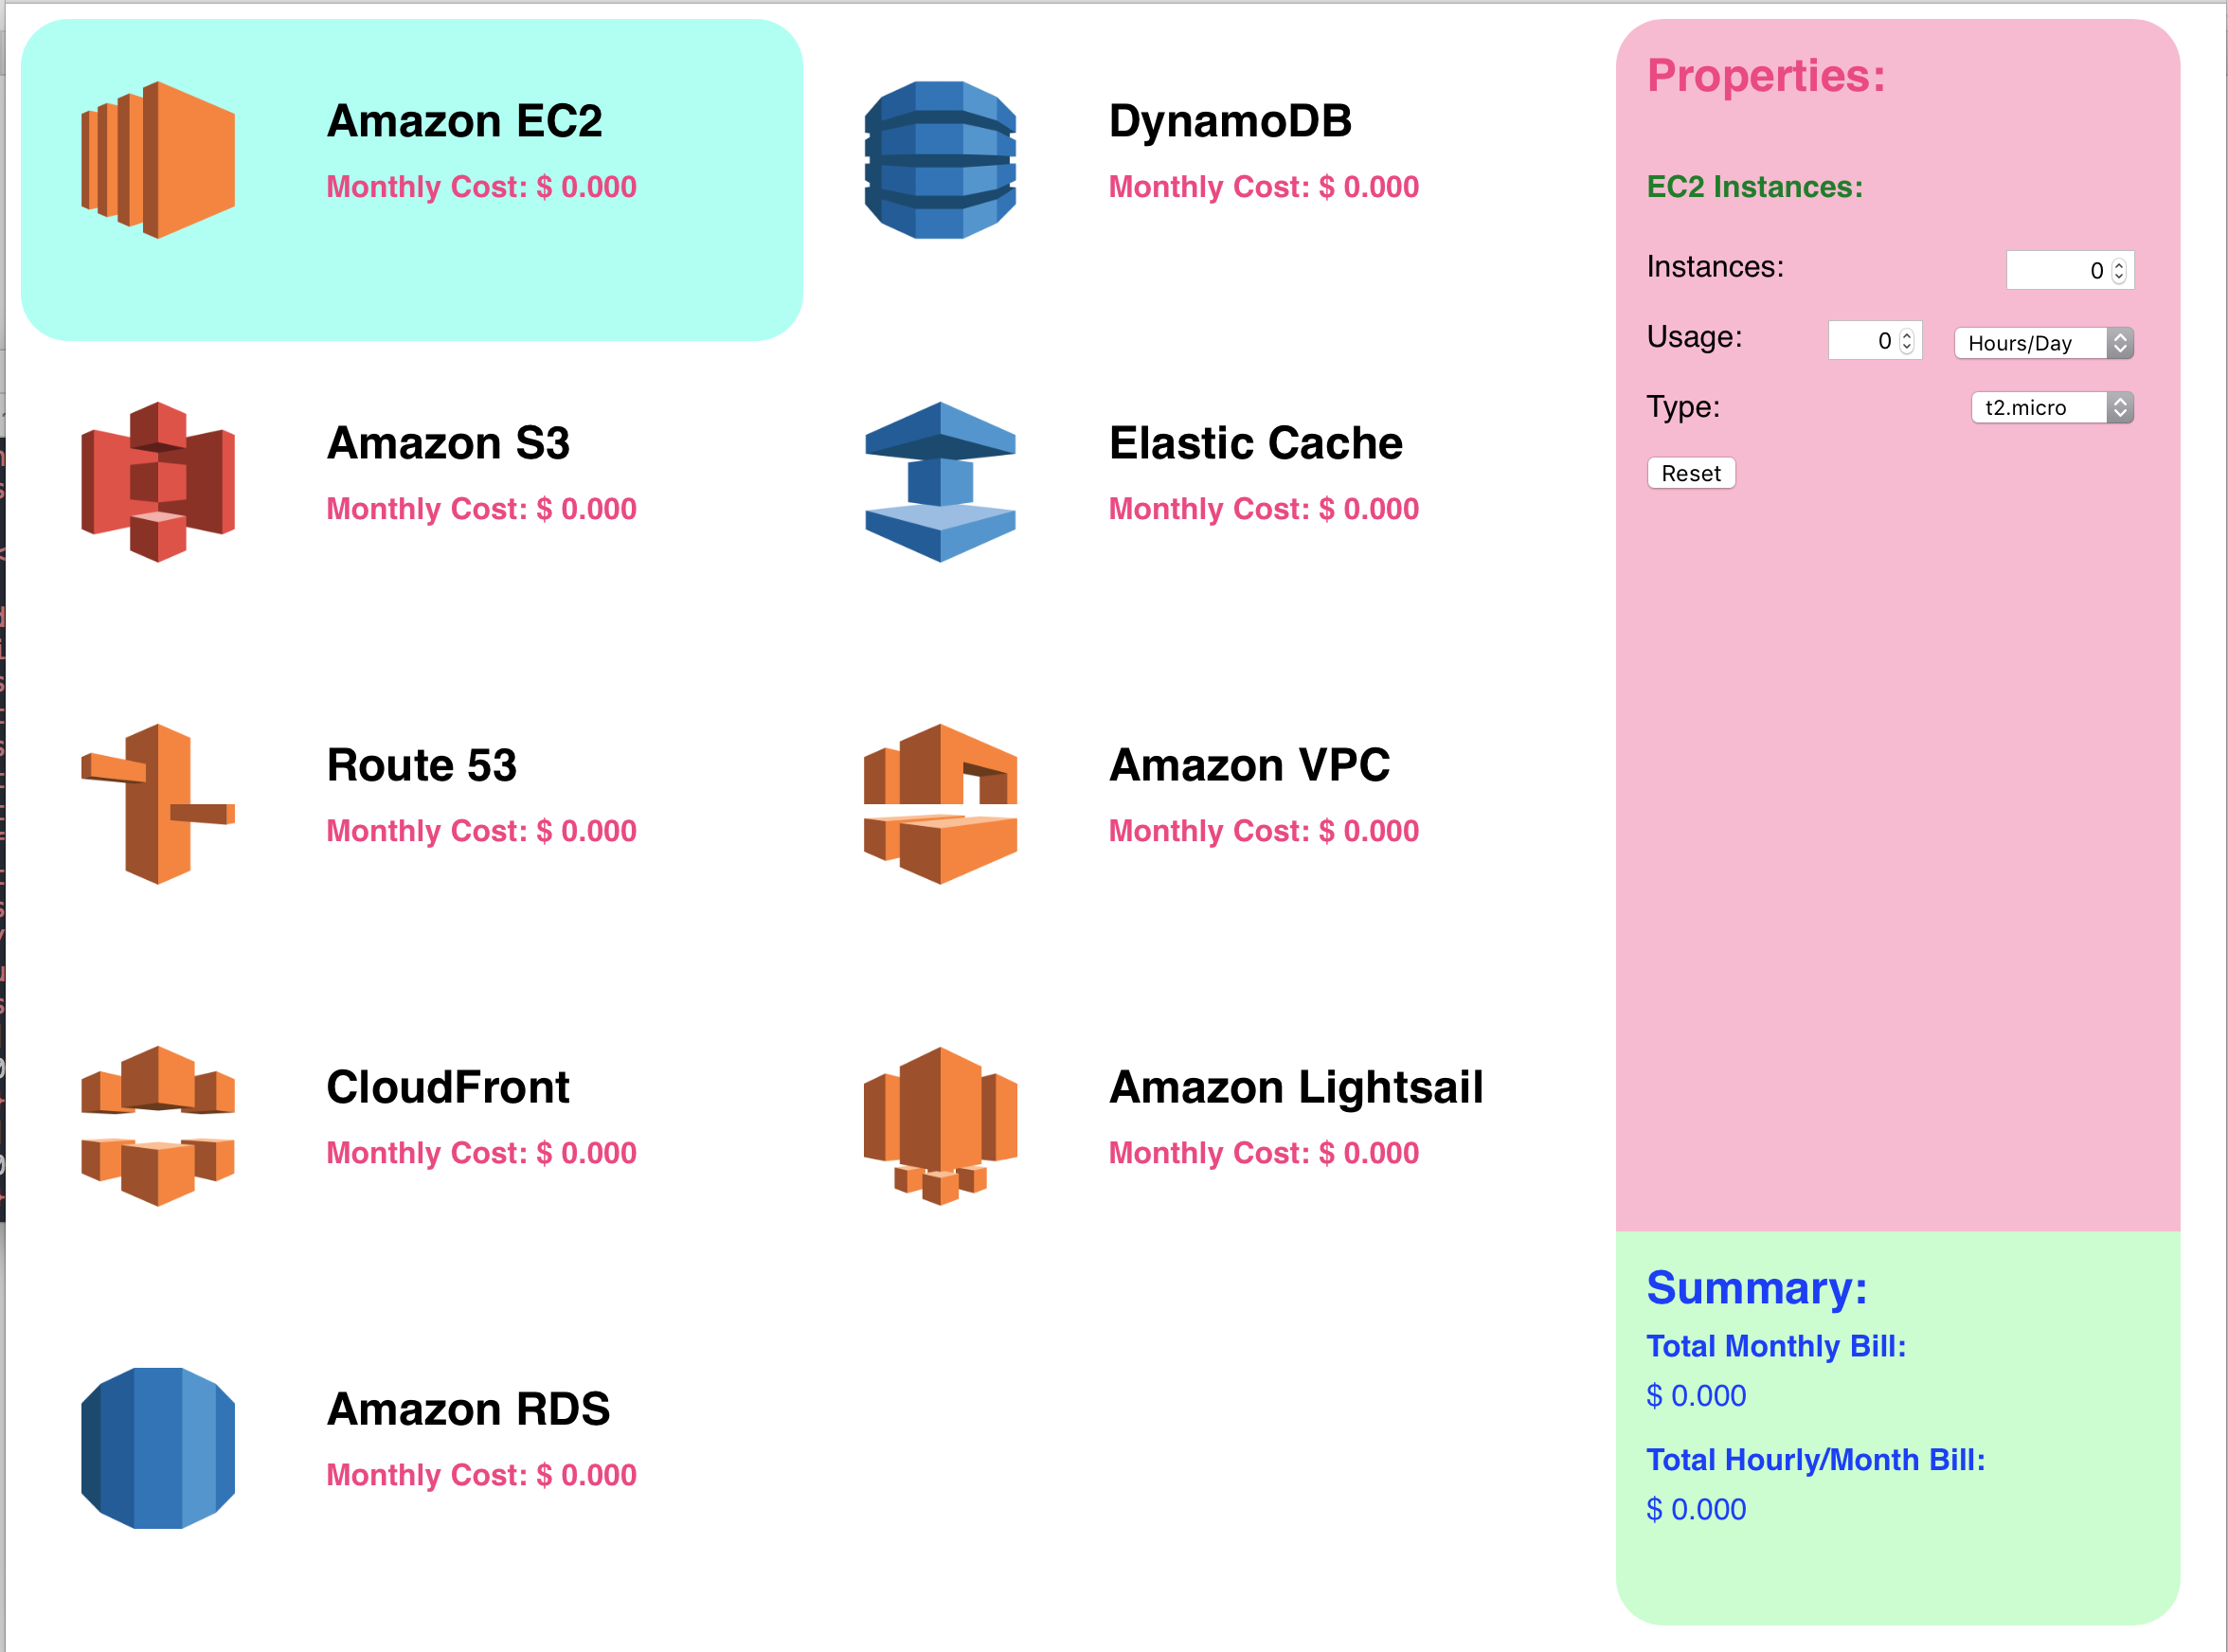
\includegraphics[width=15cm, height=10cm]{aws2.png}
  \caption[Tampilan Menu Dipilih]{Tampilan Aplikasi Saat Menu Dipilih}
  \end{figure}

  Isi kode dari midM adalah sebagai berikut:
     \begin{lstlisting}[language=Haskell]
       midM <- elClass "div" "middleMenu" $ do
             rec
              ec2 <- serviceButton "Amazon EC2" EC2 ec2dynAttrs (theDynCost rightM 1)
              s3  <- serviceButton "Amazon S3" S3 s3dynAttrs (theDynCost rightM 2)
              r53 <- serviceButton "Route 53" R53 r53dynAttrs (theDynCost rightM 3)
              cf  <- serviceButton "CloudFront" CF cfdynAttrs (theDynCost rightM 4)
              rds <- serviceButton "Amazon RDS" RDS rdsdynAttrs (theDynCost rightM 5)
              db  <- serviceButton "DynamoDB" DB dbddynAttrs (theDynCost rightM 6)
              ec  <- serviceButton "Elastic Cache" EC ecdynAttrs (theDynCost rightM 7)
              vpc <- serviceButton "Amazon VPC" VPC vpcdynAttrs (theDynCost rightM 9)
              ls  <- serviceButton "Amazon Lightsail" LS lsdynAttrs (theDynCost rightM 10)

              let 
	          ec2dynAttrs = labelAttrs <$> curSelect dynSelect EC2
	          s3dynAttrs  = labelAttrs <$> curSelect dynSelect S3
	          r53dynAttrs = labelAttrs <$> curSelect dynSelect R53
	          cfdynAttrs  = labelAttrs <$> curSelect dynSelect CF
	          rdsdynAttrs = labelAttrs <$> curSelect dynSelect RDS
	          dbddynAttrs = labelAttrs <$> curSelect dynSelect DB
	          ecdynAttrs  = labelAttrs <$> curSelect dynSelect EC
	          vpcdynAttrs = labelAttrs <$> curSelect dynSelect VPC
	          lsdynAttrs  = labelAttrs <$> curSelect dynSelect LS
              dynSelect <- holdDyn Nothing $ Just <$> leftmost [ec2, s3, r53, cf, rds, db, ec, vpc, ls]
             return dynSelect
     \end{lstlisting}
  Seperti telah dijelaskan pada bab sebelumnya bahwa tanda '($<$- )' merupakan \emph{binding arrow} dimana midM akan mengandung nilai dari hasil eksekusi kode setelah tanda '( $<$- )' yang ditandai dengan kode 'return dynSelect'. Variabel dynSelect sendiri berisikan nilai dari hasil variabel ec2, s3, r53, cf, rds, db, ec, vpc, ls dimana variabel-variable tersebut terdapat dalam sebuah list dan dijalankan oleh fungsi leftmost. Fungsi leftmost berguna untuk acuan program atas tombol mana yang ditekan terlebih dahulu oleh pengguna. Sehingga, apabila tombol pada icon ec2 ditekan, maka midM akan menghasilkan sebuah tipe data 'Dynamic t (Maybe AwsIcon)', dimana nilai dari AwsIcon pada tipe data tersebut adalah EC2.
     
  Fungsi midM kemudian mengirimkan hasil seleksi secara dinamis tersebut kedalam fungsi rightM, sehingga tampilan pada sisi kanan aplikasi akan berubah seketika setelah menu utama dipilih. Tampilan rightM adalah tampilan properties dari jasa EC2 pada AWS yang digunakan untuk munentukan hasil estimasi biaya yang harus dikeluarkan. Hasil dari kalkulasi ini akan digunakan untuk menentukan total biaya untuk ditampilkan pada summary menu dan pada setiap icon sesuai dengan properti masing-masing icon. Isi dari kode pada rightM adalah sebagai berikut:
     
   \begin{lstlisting}[language=Haskell]
    rightM <- elClass "div" "rightMenu" $ do
               el "h2" $ text "Properties: "
               rec
                ec2Prop <- ec2Properties ec2dynAttrs
                s3Prop  <- s3Properties s3dynAttrs
                r53Prop  <- r53Properties r53dynAttrs
                cfProp  <- cfProperties cfdynAttrs
                rdsProp  <- rdsProperties rdsdynAttrs
                dbProp  <- dbProperties dbdynAttrs
                ecProp  <- ecProperties ecdynAttrs
                vpcProp  <- vpcProperties vpcdynAttrs
                lsProp  <- lsProperties lsdynAttrs
      
                let 
	          ec2dynAttrs = showAttrs <$> curSelect midM EC2
	          s3dynAttrs  = showAttrs <$> curSelect midM S3
	          r53dynAttrs = showAttrs <$> curSelect midM R53
	          cfdynAttrs  = showAttrs <$> curSelect midM CF
	          rdsdynAttrs = showAttrs <$> curSelect midM RDS
	          dbdynAttrs  = showAttrs <$> curSelect midM DB
	          ecdynAttrs  = showAttrs <$> curSelect midM EC
                  vpcdynAttrs = showAttrs <$> curSelect midM VPC
	          lsdynAttrs  = showAttrs <$> curSelect midM LS
               return [ (1 , ec2Prop)
	              , (2 , s3Prop )
	              , (3 , r53Prop)
		      , (4 , cfProp )
		      , (5 , rdsProp)
		      , (6 , dbProp )
		      , (7 , ecProp )
		      , (8 , vpcProp)
		      , (9 , lsProp )
		      ]
   \end{lstlisting}

   Dari kode diatas, properti dari masing-masing tombol icon pada menu midM ditentukan oleh atribut dari
  \begin{lstlisting}[language=HTML]
  <div class="rightProp" id="EC2" style="display:none">...</div>
  \end{lstlisting}
dimana display tersebut akan muncul dengan diubahnya 'none' menjadi 'inline-flex' apabila hasil dari fungsi 'curSelect' yang diaplikasikan kepada variabel midM dan masing-masing icon bernilai True. Sehingga fungsi:
  \begin{lstlisting}[language=Haskell]
  showAttrs :: Bool -> Map.Map T.Text T.Text
  showAttrs b = "style" =: ("display: " <> display' b)
  where
    display' True = "inline-flex"
    display' _    = "none"
  \end{lstlisting}
  yang diaplikasikan terhadap hasil dari fungsi curSelect tersebut merubah atribut \emph{style} dengan nilai \emph{display} secara dinamis sesuai dengan keadaan dimana tombol icon AWS pada menu midM sedang ditekan. Dengan demikian, setiap properti yang diubah akan membawa suatu hasil yang berbeda sesuai keadaan terakhir nilai dari masing-masing properti tersebut. Variabel rightM akan membawa sebuah nilai hasil dari perhitungan masing-masing properti pada icon AWS dengan melakukan pemetaan berupa hashmap, yaitu sebuah pemetaan yang setiap nilai dari suatu variabel ditandai dengan kunci-kunci yang mencirikan variabel tersebut. Seperti contoh pada kode sebagai berikut:
    \begin{lstlisting}[language=Haskell]
               return [ (1 , ec2Prop)
	              , (2 , s3Prop )
	              , (3 , r53Prop)
		      , (4 , cfProp )
		      , (5 , rdsProp)
		      , (6 , dbProp )
		      , (7 , ecProp )
		      , (8 , vpcProp)
		      , (9 , lsProp )
		      ]
    \end{lstlisting}
    yaitu rightM akan membawa sebuah nilai dinamis (\emph{dynamic values} yang memiliki kunci dari 1 sampai 9 untuk menandakan masing-masing properti (misalnya: kunci 1 untuk variabel ec2Prop, yaitu hasil dari perhitungan properti pada saat tombol ikon EC2 ditekan). Nilal kembalian ini akan digunakan oleh midM untuk menampilkan total biaya pada setiap ikonnya. Hal ini dimungkinkan karena adanya fungsi 'rec' pada notasi 'do' pada fungsi bodyElement.

   Hasil dari kalkulasi tersebut salah satunya akan ditampilkan pada menu summary yang terletak di sisi kanan bawah pada gambar diatas. Hasil kalkulasi tersebut diperoleh dari penjumlahan seluruh properti yang telah dihitung sesuai dengan ketentuan harga yang diberikan oleh situs dokumentasi AWS yang resmi. Isi dari kode pada 'elClass ``div'' "summaryMenu"  adalah sebagai berikut:
   \begin{lstlisting}[language=Haskell]
let
        resultList = (fmap . fmap) readDouble (Map.elems $ Map.fromList rightM)
	starter = readDouble <$> (constDyn "0")
	joined = join $ foldM foldTheCost starter resultList
      el "h2" $ text "Summary: "
      el "h4" $ text "Total Monthly Bill: "
      -- This is how foldM will work:
      --
      -- foldM f Dynamic t 0 [Dynamic t 5, Dynamic t 6]
      -- do
      --   a2 <- f (Dynamic t 0) (Dynamic t 5)
      --   a3 <- f (Dynamic t 5) (Dynamic t 6)
      --
      el "p" $ dynText $ (constDyn "$ ") <> (toText <$> (join $ foldM foldTheCost starter resultList))
      el "h4" $ text "Total Hourly/Month Bill: "
      el "p" $ dynText $ (constDyn "$ ") <> (toText <$> ((/720) <$> joined))
   \end{lstlisting}
   
  Kode yang menghitung total keseluruhan dari biaya masing-masing menu adalah:
     \begin{lstlisting}[language=Haskell]
  el "p" $ dynText $ (constDyn "$ ") <> (toText <$> (join $ foldM foldTheCost starter resultList))
     \end{lstlisting}
dimana berguna untuk menggabungkan perhitungan dari setiap hasil kalkulasi yang dilakukan secara dinamis melalui fungsi foldTheCost. Sehingga, perubahan yang terjadi pada properti dari masing-masing menu yang secara seketika diperbaharui akan turut melakukan pembaharuan terhadap nilai jumlah biaya yang tertera pada teks "Total Hourly/Month Bill" dan "Total Monthly Bill: ".

     
\section{Hasil Uji Coba}
Hasil uji coba pada penelitian ilmiah ini adalah sebagai berikut:
\begin{enumerate}
\item Tampilan properti jasa AWS telah sesuai dengan ikon yang aktif pada menu utama
\item Setiap penambahan / perubahan pada properti dari setiap ikon aktif akan merubah tampilan "Monthly Cost pada masing-masing ikon pada menu utama dan pada summary menu
\item Perhitungan harga telah sesuai dengan dokumentasi harga dari situs resmi Amazon AWS di \url{amazon.com}
\item Jumlah total harga pada summary menu telah sama dengan hasil penjumlahan harga dari masing-masing ikon pada menu utama
  
\end{enumerate}


     
\end{document}
